\documentclass[12pt]{article}
\usepackage{amsfonts}
\usepackage{comment}
\usepackage{tikz}
\usetikzlibrary{arrows,automata}
\begin{document}

\noindent
Jason Downing \\
Email: jason\_downing@student.uml.edu \\
Foundations of Computer Science \\
Homework \#2 - Chapter 1: DFA, NFA\\
10/6/2016 \\

\noindent
1.3 \\
The formal description of a DFA M is \{q1, q2, q3, q4, q5 \}, \\
\{u, d\}, $\delta$, q3 , \{q3\}, where $\delta$  is given by the following table:
\begin{center}
\begin{tabular}{ c | c c }
 & u & d \\
\hline
 q1 & q1 & q2 \\ 
 q2 & q1 & q3 \\  
 q3 & q2 & q4 \\
 q4 & q3 & q5 \\
 q5 & q4 & q5
\end{tabular}
\end{center}

\noindent
Initial state is q3, so that is where the machine will start. \\
We can use the table to create the nodes, and connect them as needed. \\
The accepted state is q3 so we will mark that with a double circle to \\
show that as the accepted state of the machine. \\

\begin{center}
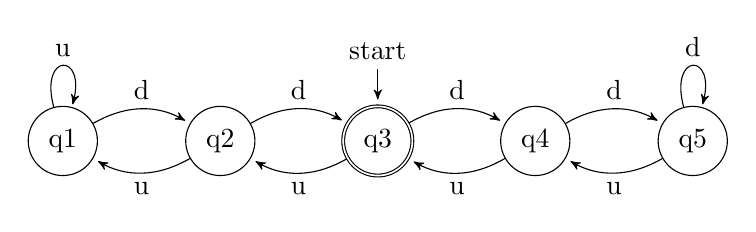
\begin{tikzpicture}[>=stealth',shorten >=2pt, auto, node distance=2cm]
	% Nodes {q1, q2, q3, q4, q5}
	\node [state] 											(q1) 				{q1};
	\node [state] 											(q2) [right of=q1]  {q2};
	\node [state, initial, initial where=above, accepting]  (q3) [right of=q2]  {q3};
	\node [state]											(q4) [right of=q3]  {q4};
	\node [state]   										(q5) [right of=q4]  {q5};

	% Paths
	\path [->] 	(q1) edge [loop above] node	{u}	(q1)
	            (q1) edge [bend left]  node {d} (q2)
				(q2) edge [bend left]  node {u} (q1)
				(q2) edge [bend left]  node {d} (q3)
				(q3) edge [bend left]  node {u} (q2)
				(q3) edge [bend left]  node {d} (q4)
				(q4) edge [bend left]  node {u} (q3)
				(q4) edge [bend left]  node {d} (q5)
				(q5) edge [bend left]  node {u} (q4)
				(q5) edge [loop above] node	{d}	(q5);
				
\end{tikzpicture} \\
\end{center}


\noindent
1.4: a, c, e, f, g \\
\indent
For all parts, $\sum = \{a, b\} $ \\

a. \{ w$|$ w has at least three a\textsc{\char13}s \}
\begin{center}
	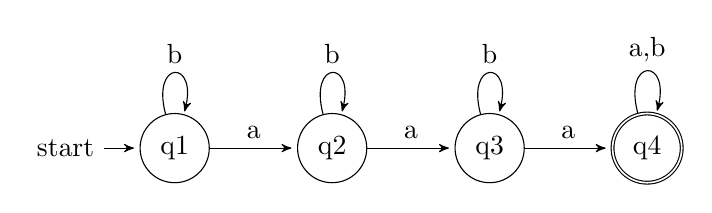
\begin{tikzpicture}[>=stealth',shorten >=2pt, auto, node distance=2cm]
	% Nodes {q1, q2, q3, q4, q5, etc}
	\node [state, initial] 		(q1) 				 {q1};
	\node [state] 				(q2)  [right of=q1]  {q2};
	\node [state]   			(q3)  [right of=q2]  {q3};
	\node [state, accepting]	(q4)  [right of=q3]  {q4};
	
	% Paths
	\path [->] 	(q1) edge 				node	{a}		(q2);
	\path [->] 	(q1) edge [loop above] 	node	{b}		(q1);
	\path [->] 	(q2) edge 				node	{a}		(q3);
	\path [->] 	(q2) edge [loop above] 	node	{b}		(q2);
	\path [->] 	(q3) edge 				node	{a}		(q4);
	\path [->] 	(q3) edge [loop above] 	node	{b}		(q3);
	\path [->] 	(q4) edge [loop above] 	node	{a,b}	(q4);
	
	\end{tikzpicture} \\
\end{center}

\{ w$|$ w has at least two b\textsc{\char13}s \}
\begin{center}
	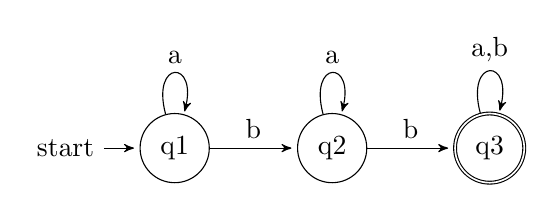
\begin{tikzpicture}[>=stealth',shorten >=2pt, auto, node distance=2cm]
	% Nodes {q1, q2, q3, q4, q5, etc}
	\node [state, initial] 		(q1) 				 {q1};
	\node [state] 				(q2)  [right of=q1]  {q2};
	\node [state, accepting]	(q3)  [right of=q2]  {q3};
	
	% Paths
	\path [->] 	(q1) edge 				node	{b}		(q2);
	\path [->] 	(q1) edge [loop above] 	node	{a}		(q1);
	\path [->] 	(q2) edge 				node	{b}		(q3);
	\path [->] 	(q2) edge [loop above] 	node	{a}		(q2);
	\path [->] 	(q3) edge [loop above] 	node	{a,b}	(q3);
	
	\end{tikzpicture} \\
\end{center}

\{w$|$ w has at least three a’s and at least two b’s\}
\begin{center}
	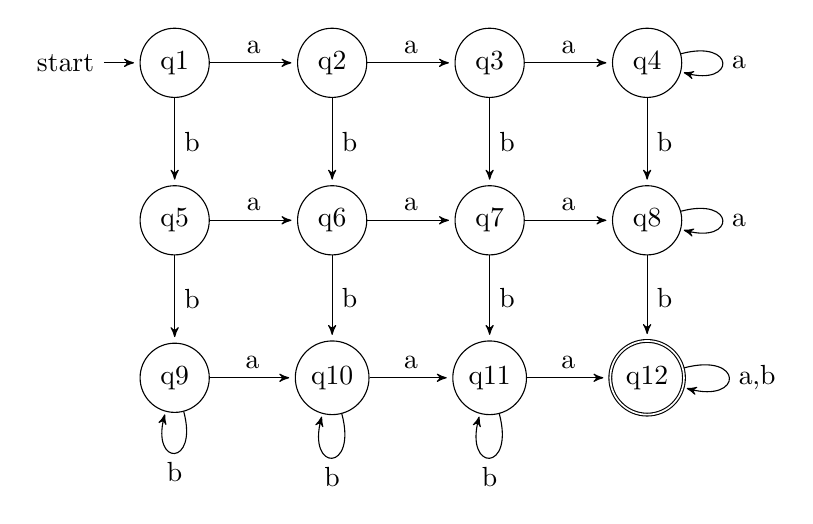
\begin{tikzpicture}[>=stealth',shorten >=2pt, auto, node distance=2cm]
	% Nodes {q1, q2, q3, q4, q5, etc}
	\node [state, initial] 		(q1) 				 {q1};
	\node [state] 				(q2)  [right of=q1]  {q2};
	\node [state]   			(q3)  [right of=q2]  {q3};
	\node [state]				(q4)  [right of=q3]  {q4};
	\node [state]   			(q5)  [below of=q1]  {q5};
	\node [state]   			(q6)  [below of=q2]  {q6};
	\node [state]   			(q7)  [below of=q3]  {q7};
	\node [state]   			(q8)  [below of=q4]  {q8};
	\node [state]   			(q9)  [below of=q5]  {q9};
	\node [state]   			(q10) [below of=q6]  {q10};
	\node [state]   			(q11) [below of=q7]  {q11};
	\node [state, accepting]   	(q12) [below of=q8]  {q12};
	
	% Paths for first row
	\path [->] 	(q1) edge 				node	{a}	(q2);
	\path [->] 	(q1) edge 				node	{b}	(q5);
	\path [->] 	(q2) edge 				node	{a}	(q3);
	\path [->] 	(q2) edge 				node	{b}	(q6);
	\path [->] 	(q3) edge 				node	{a}	(q4);
	\path [->] 	(q3) edge 				node	{b}	(q7);
	\path [->] 	(q4) edge [loop right] 	node	{a}	(q4);
	\path [->] 	(q4) edge 				node	{b}	(q8);
	
	% Paths for second row
	\path [->] 	(q5) edge			 	node	{a}	(q6);
	\path [->] 	(q5) edge 				node	{b}	(q9);
	\path [->] 	(q6) edge 				node	{a}	(q7);
	\path [->] 	(q6) edge 				node	{b}	(q10);
	\path [->] 	(q7) edge 				node	{a}	(q8);
	\path [->] 	(q7) edge 				node	{b}	(q11);
	\path [->] 	(q8) edge [loop right] 	node	{a}	(q8);
	\path [->] 	(q8) edge 				node	{b}	(q12);
	
	% Paths for third row
	\path [->] 	(q9)  edge 				node  {a} 	(q10);
	\path [->] 	(q9)  edge [loop below] node  {b} 	(q9);
	\path [->] 	(q10) edge 				node  {a} 	(q11);
	\path [->] 	(q10) edge [loop below] node  {b} 	(q10);
	\path [->] 	(q11) edge 				node  {a} 	(q12);
	\path [->] 	(q11) edge [loop below]	node  {b} 	(q11);
	\path [->] 	(q12) edge [loop right] node  {a,b}	(q12);

	\end{tikzpicture} \\
\end{center}

c. \{ w$|$ w has an even number of a\textsc{\char13}s \}
\begin{center}
	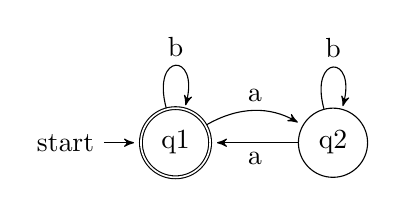
\begin{tikzpicture}[>=stealth',shorten >=2pt, auto, node distance=2cm]
	% Nodes {q1, q2, q3, q4, q5, etc}
	\node [state, initial, accepting] 		(q1) 				 {q1};
	\node [state] 							(q2)  [right of=q1]  {q2};
	
	% Paths
	\path [->] 	(q1) edge [bend left]	node	{a}		(q2);
	\path [->] 	(q1) edge [loop above] 	node	{b}		(q1);
	\path [->] 	(q2) edge				node	{a}		(q1);
	\path [->] 	(q2) edge [loop above] 	node	{b}		(q2);
	
	\end{tikzpicture} \\
\end{center}

\{ w$|$ w has one or two b\textsc{\char13}s \}
\begin{center}
	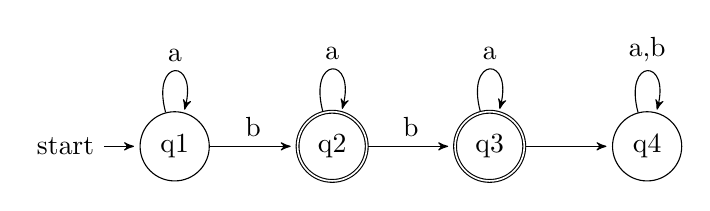
\begin{tikzpicture}[>=stealth',shorten >=2pt, auto, node distance=2cm]
	% Nodes {q1, q2, q3, q4, q5, etc}
	\node [state, initial] 		(q1) 				 {q1};
	\node [state, accepting] 	(q2)  [right of=q1]  {q2};
	\node [state, accepting]    (q3)  [right of=q2]  {q3};
	\node [state]				(q4)  [right of=q3]  {q4};
	
	% Paths
	\path [->] 	(q1) edge 				node	{b}		(q2);
	\path [->] 	(q1) edge [loop above] 	node	{a}		(q1);
	\path [->] 	(q2) edge 				node	{b}		(q3);
	\path [->] 	(q2) edge [loop above] 	node	{a}		(q2);
	\path [->] 	(q3) edge 				node	{}		(q4);
	\path [->] 	(q3) edge [loop above] 	node	{a}		(q3);
	\path [->] 	(q4) edge [loop above] 	node	{a,b}	(q4);
	
	\end{tikzpicture} \\
\end{center}

\{ w$|$ w has an even number of a\textsc{\char13}s
and one or two b\textsc{\char13}s \}
\begin{center}
	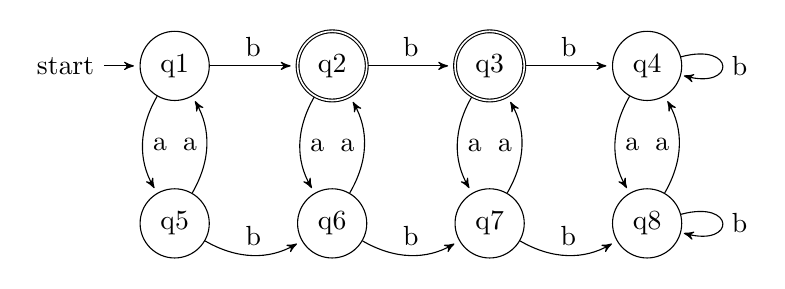
\begin{tikzpicture}[>=stealth',shorten >=2pt, auto, node distance=2cm]
	% Nodes {q1, q2, q3, q4, q5, etc}
	\node [state, initial] 		(q1) 				 {q1};
	\node [state, accepting] 	(q2)  [right of=q1]  {q2};
	\node [state, accepting]    (q3)  [right of=q2]  {q3};
	\node [state]				(q4)  [right of=q3]  {q4};
	\node [state]				(q5)  [below of=q1]  {q5};
	\node [state]				(q6)  [below of=q2]  {q6};
	\node [state]				(q7)  [below of=q3]  {q7};
	\node [state]				(q8)  [below of=q4]  {q8};
	
	% Paths
	\path [->] 	(q1) edge 				node	{b}		(q2);
	\path [->] 	(q1) edge [bend right]	node	{a}		(q5);
	\path [->] 	(q2) edge 				node	{b}		(q3);
	\path [->] 	(q2) edge [bend right]	node	{a}		(q6);
	\path [->] 	(q3) edge 				node	{b}		(q4);
	\path [->] 	(q3) edge [bend right]	node	{a}		(q7);
	\path [->] 	(q4) edge [loop right] 	node	{b}		(q4);
	\path [->] 	(q4) edge [bend right]	node	{a}		(q8);
	\path [->] 	(q5) edge [bend right]	node	{a}		(q1);
	\path [->] 	(q5) edge [bend right]	node	{b}		(q6);
	\path [->] 	(q6) edge [bend right]	node	{a}		(q2);
	\path [->] 	(q6) edge [bend right]	node	{b}		(q7);
	\path [->] 	(q7) edge [bend right]	node	{a}		(q3);
	\path [->] 	(q7) edge [bend right]	node	{b}		(q8);
	\path [->] 	(q8) edge [bend right]	node	{a}		(q4);
	\path [->] 	(q8) edge [loop right]	node	{b}		(q8);
	
	\end{tikzpicture} \\
\end{center}

e. \{ w$|$ w starts with an a \}
\begin{center}
	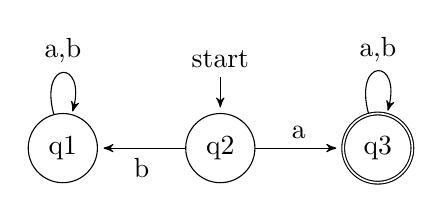
\begin{tikzpicture}[>=stealth',shorten >=2pt, auto, node distance=2cm]
	% Nodes {q1, q2, q3, q4, q5, etc}
	\node [state] 									(q1) 				 {q1};
	\node [state, initial, initial where=above] 	(q2)  [right of=q1]  {q2};
	\node [state, accepting]						(q3)  [right of=q2]  {q3};
	
	% Paths
	\path [->] 	(q1) edge [loop above] 	node	{a,b}	(q1);
	\path [->] 	(q2) edge 				node	{b}		(q1);
	\path [->] 	(q2) edge 				node	{a}		(q3);
	\path [->] 	(q3) edge [loop above] 	node	{a,b}	(q3);
	
	\end{tikzpicture} \\
\end{center}

\{ w$|$ w has at most one b \}
\begin{center}
	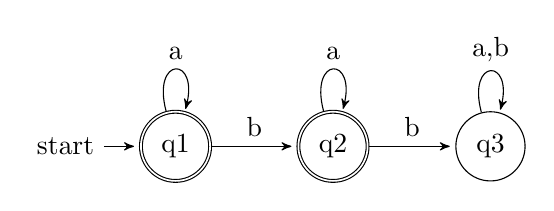
\begin{tikzpicture}[>=stealth',shorten >=2pt, auto, node distance=2cm]
	% Nodes {q1, q2, q3, q4, q5, etc}
	\node [state, initial,accepting] 	(q1) 				 {q1};
	\node [state, accepting] 			(q2)  [right of=q1]  {q2};
	\node [state]						(q3)  [right of=q2]  {q3};
	
	% Paths
	\path [->] 	(q1) edge [loop above] 	node	{a}     (q1);
	\path [->] 	(q1) edge 				node	{b}		(q2);
    \path [->] 	(q2) edge [loop above] 	node	{a}     (q2);
	\path [->] 	(q2) edge 				node	{b}		(q3);
	\path [->] 	(q3) edge [loop above] 	node	{a,b}	(q3);
	
	\end{tikzpicture} \\
\end{center}

\{ w$|$ w starts with an a and has at most one b \}

% TODO fix this
not sure how to do this yet... dotted lines and circles are ??? \\

f. \{ w$|$ w has an odd number of a\textsc{\char13}s \}
\begin{center}
    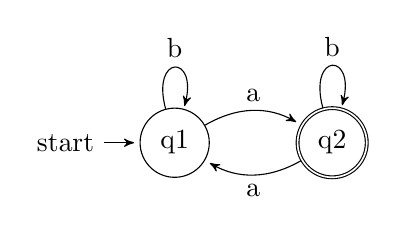
\begin{tikzpicture}[>=stealth',shorten >=2pt, auto, node distance=2cm]
    % Nodes {q1, q2, q3, q4, q5, etc}
    \node [state, initial] 	    (q1) 				 {q1};
    \node [state, accepting]    (q2)  [right of=q1]  {q2};
    
    % Paths
    \path [->] 	(q1) edge [loop above] 	node	{b}     (q1);
    \path [->] 	(q1) edge [bend left]   node	{a}		(q2);
    \path [->] 	(q2) edge [loop above] 	node	{b}     (q2);
    \path [->] 	(q2) edge [bend left] 	node	{a}		(q1);
    
    \end{tikzpicture} \\
\end{center}

\{ w$|$ w ends with a b \}
\begin{center}
    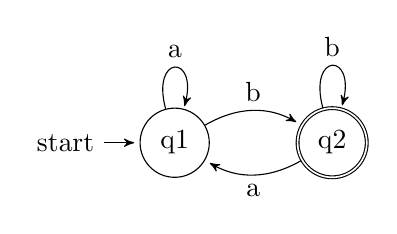
\begin{tikzpicture}[>=stealth',shorten >=2pt, auto, node distance=2cm]
    % Nodes {q1, q2, q3, q4, q5, etc}
    \node [state, initial] 	    (q1) 				 {q1};
    \node [state, accepting]    (q2)  [right of=q1]  {q2};
    
    % Paths
    \path [->] 	(q1) edge [loop above] 	node	{a}     (q1);
    \path [->] 	(q1) edge [bend left]   node	{b}		(q2);
    \path [->] 	(q2) edge [loop above] 	node	{b}     (q2);
    \path [->] 	(q2) edge [bend left] 	node	{a}		(q1);
    
    \end{tikzpicture} \\
\end{center}

\{ w$|$ w has an odd number of a\textsc{\char13}s and ends with a b \}
\begin{center}
    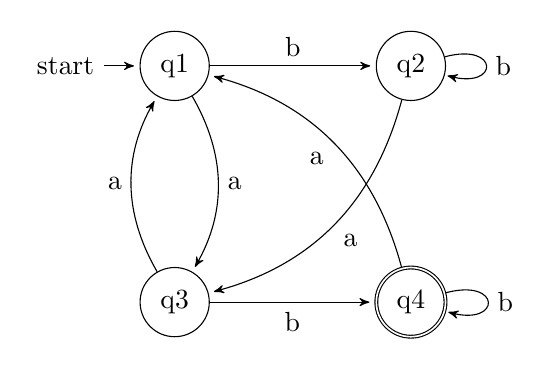
\begin{tikzpicture}[>=stealth',shorten >=2pt, auto, node distance=3cm]
    % Nodes {q1, q2, q3, q4, q5, etc}
    \node [state, initial] 	    (q1) 				 {q1};
    \node [state] 	            (q2)  [right of=q1]  {q2};
    \node [state] 	            (q3)  [below of=q1]  {q3};
    \node [state, accepting]    (q4)  [below of=q2]  {q4};
    
    % Paths
    \path [->] 	(q1) edge           	node	        {b}     (q2);
    \path [->] 	(q1) edge [bend left]   node	        {a}     (q3);
    \path [->] 	(q2) edge [loop right] 	node	        {b}     (q2);
    \path [->] 	(q2) edge [bend left]	node	        {a}		(q3);
    \path [->] 	(q3) edge [bend left]   node	        {a}     (q1);
    \path [->] 	(q3) edge               node [below]	{b}     (q4);
    \path [->] 	(q4) edge [loop right] 	node	        {b}     (q4);
    \path [->] 	(q4) edge [bend right]	node	        {a}		(q1);
    
    \end{tikzpicture} \\
\end{center}

g. \{ w$|$ w has even length \} \\
\begin{center}
    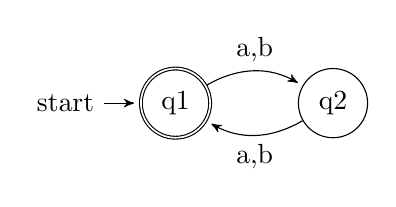
\begin{tikzpicture}[>=stealth',shorten >=2pt, auto, node distance=2cm]
    % Nodes {q1, q2, q3, q4, q5, etc}
    \node [state, initial, accepting] 	(q1) 				 {q1};
    \node [state]                       (q2)  [right of=q1]  {q2};
    
    % Paths
    \path [->] 	(q1) edge [bend left]   node	{a,b}		(q2);
    \path [->] 	(q2) edge [bend left] 	node	{a,b}		(q1);
    
    \end{tikzpicture} \\
\end{center}

\{ w$|$ w has an odd number of a\textsc{\char13}s \}
\begin{center}
    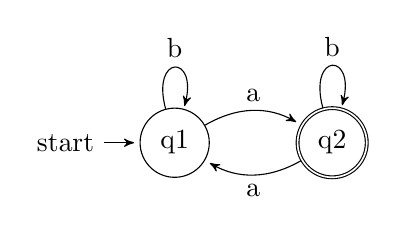
\begin{tikzpicture}[>=stealth',shorten >=2pt, auto, node distance=2cm]
    % Nodes {q1, q2, q3, q4, q5, etc}
    \node [state, initial] 	  (q1) 				   {q1};
    \node [state, accepting]  (q2)  [right of=q1]  {q2};
    
    % Paths
    \path [->] 	(q1) edge [bend left]   node	{a}		(q2);
    \path [->] 	(q1) edge [loop above] 	node	{b}     (q1);
    \path [->] 	(q2) edge [bend left] 	node	{a}		(q1);
    \path [->] 	(q2) edge [loop above] 	node	{b}     (q2);
    
    \end{tikzpicture} \\
\end{center}

\{ w$|$ w has even length and an odd number of a\textsc{\char13}s \}
\begin{center}
    \begin{tikzpicture}[>=stealth',shorten >=2pt, auto, node distance=3cm]
    % Nodes {q1, q2, q3, q4, q5, etc}
    \node [state, initial] 	  (q1) 				   {q1};
    \node [state] 	          (q2) 	[right of=q2]  {q2};
    \node [state] 	          (q3) 	[below of=q1]  {q3};
    \node [state, accepting]  (q4)  [below of=q2]  {q4};
    
    % Paths
    \path [->] 	(q1) edge [bend left]   node	        {b}		(q2);
    \path [->] 	(q1) edge [bend left] 	node	        {a}     (q3);
    \path [->] 	(q2) edge [bend left] 	node [above]	{b}		(q1);
    \path [->] 	(q2) edge [bend left] 	node	        {a}     (q4);
    \path [->] 	(q3) edge [bend left] 	node	        {a}     (q1);
    \path [->] 	(q3) edge [bend left] 	node [below]    {b}     (q4);
    \path [->] 	(q4) edge [bend left] 	node	        {b}     (q3);
    \path [->] 	(q4) edge [bend left] 	node	        {a}     (q2);
    
    \end{tikzpicture} \\
\end{center}

\noindent
1.5: c, d, e, f, g, h \\
\indent
For all parts, $\sum = \{a, b\} $ \\

c. \{ w$|$ w contains neither the substrings ab nor ba \} \\

Simpler language \\
\begin{center}
    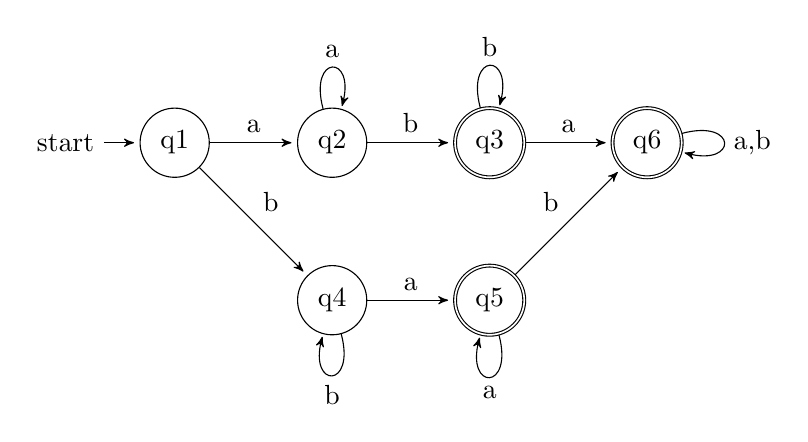
\begin{tikzpicture}[>=stealth',shorten >=2pt, auto, node distance=2cm]
    % Nodes {q1, q2, q3, q4, q5, etc}
    \node [state, initial] 		(q1) 				 {q1};
    \node [state] 	            (q2)  [right of=q1]  {q2};
    \node [state, accepting]    (q3)  [right of=q2]  {q3};
    \node [state]	            (q4)  [below of=q2]  {q4};
    \node [state, accepting]	(q5)  [below of=q3]  {q5};
    \node [state, accepting]	(q6)  [right of=q3]  {q6};
    
    % Paths
    \path [->] 	(q1) edge 				node	{a}		(q2);
    \path [->] 	(q1) edge 				node	{b}		(q4);
    \path [->] 	(q2) edge 				node	{b}		(q3);
    \path [->] 	(q2) edge [loop above]	node	{a}		(q2);
    \path [->] 	(q3) edge 				node	{a}		(q6);
    \path [->] 	(q3) edge [loop above]	node	{b}		(q3);
    \path [->] 	(q4) edge 				node	{a}		(q5);
    \path [->] 	(q4) edge [loop below]	node	{b}		(q4);
    \path [->] 	(q5) edge 				node	{b}		(q6);
    \path [->] 	(q5) edge [loop below]	node	{a}		(q5);
    \path [->] 	(q6) edge [loop right]	node	{a,b}	(q6);
    
    \end{tikzpicture} \\
\end{center}

Language given. \\
\begin{center}
    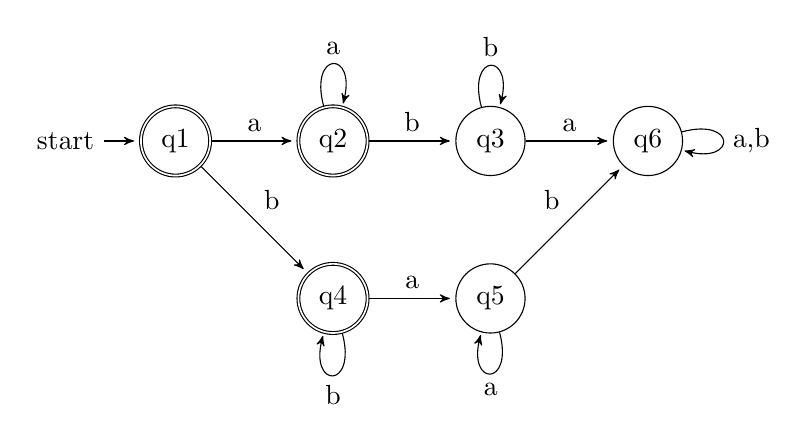
\begin{tikzpicture}[>=stealth',shorten >=2pt, auto, node distance=2cm]
    % Nodes {q1, q2, q3, q4, q5, etc}
    \node [state, initial, accepting] 		(q1) 				 {q1};
    \node [state, accepting] 	            (q2)  [right of=q1]  {q2};
    \node [state]                           (q3)  [right of=q2]  {q3};
    \node [state, accepting]	            (q4)  [below of=q2]  {q4};
    \node [state]	                        (q5)  [below of=q3]  {q5};
    \node [state]	                        (q6)  [right of=q3]  {q6};
    
    % Paths
    \path [->] 	(q1) edge 				node	{a}		(q2);
    \path [->] 	(q1) edge 				node	{b}		(q4);
    \path [->] 	(q2) edge 				node	{b}		(q3);
    \path [->] 	(q2) edge [loop above]	node	{a}		(q2);
    \path [->] 	(q3) edge 				node	{a}		(q6);
    \path [->] 	(q3) edge [loop above]	node	{b}		(q3);
    \path [->] 	(q4) edge 				node	{a}		(q5);
    \path [->] 	(q4) edge [loop below]	node	{b}		(q4);
    \path [->] 	(q5) edge 				node	{b}		(q6);
    \path [->] 	(q5) edge [loop below]	node	{a}		(q5);
    \path [->] 	(q6) edge [loop right]	node	{a,b}	(q6);
    
    \end{tikzpicture} \\
\end{center}

d. \{ w$|$ w is any string not in a*b* \} \\

Simpler language \\
\begin{center}
    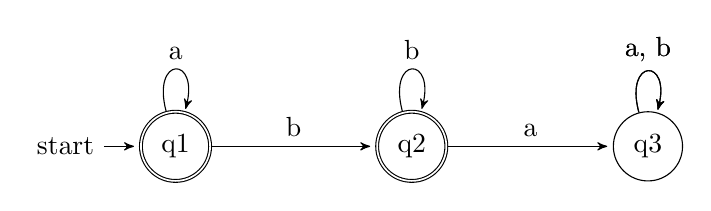
\begin{tikzpicture}[>=stealth',shorten >=2pt, auto, node distance=3cm]
    % Nodes {q1, q2, q3, q4, q5, etc}
    \node [state, initial, accepting] 		(q1) 				 {q1};
    \node [state, accepting] 	            (q2)  [right of=q1]  {q2};
    \node [state]                           (q3)  [right of=q2]  {q3};
    
    % Paths
    \path [->] 	(q1) edge 				node	{b}		(q2);
    \path [->] 	(q1) edge [loop above] 	node	{a}	    (q1);
    \path [->] 	(q2) edge 				node	{a}		(q3);
    \path [->] 	(q2) edge [loop above] 	node	{b}	    (q2);
    \path [->] 	(q3) edge [loop above] 	node	{a, b}	(q3);
    \path [->] 	(q3) edge [loop above] 	node	{a, b}	(q3);
    
    \end{tikzpicture} \\
\end{center}

Language given \\
\begin{center}
    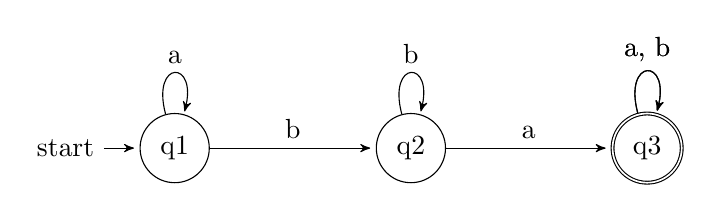
\begin{tikzpicture}[>=stealth',shorten >=2pt, auto, node distance=3cm]
    % Nodes {q1, q2, q3, q4, q5, etc}
    \node [state, initial] 		(q1) 				 {q1};
    \node [state] 	            (q2)  [right of=q1]  {q2};
    \node [state, accepting]    (q3)  [right of=q2]  {q3};
    
    % Paths
    \path [->] 	(q1) edge 				node	{b}		(q2);
    \path [->] 	(q1) edge [loop above] 	node	{a}	    (q1);
    \path [->] 	(q2) edge 				node	{a}		(q3);
    \path [->] 	(q2) edge [loop above] 	node	{b}	    (q2);
    \path [->] 	(q3) edge [loop above] 	node	{a, b}	(q3);
    \path [->] 	(q3) edge [loop above] 	node	{a, b}	(q3);
    
    \end{tikzpicture} \\
\end{center}

e. \{ w$|$ w is any string not in (ab\textsuperscript{+})* \} \\

Simpler language
\begin{center}
    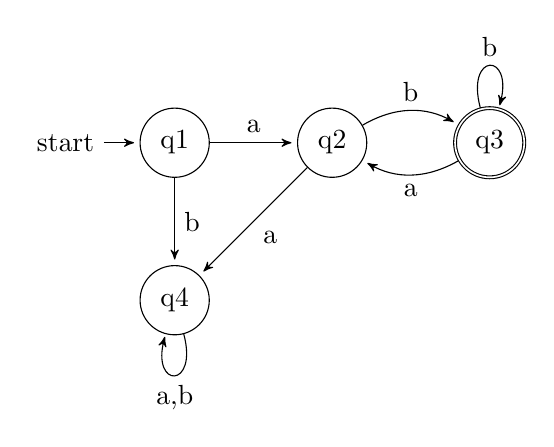
\begin{tikzpicture}[>=stealth',shorten >=2pt, auto, node distance=2cm]
    % Nodes {q1, q2, q3, q4, q5, etc}
    \node [state, initial] 		(q1) 				 {q1};
    \node [state] 	            (q2)  [right of=q1]  {q2};
    \node [state, accepting]    (q3)  [right of=q2]  {q3};
    \node [state]				(q4)  [below of=q1]  {q4};
    
    % Paths
    \path [->] 	(q1) edge 				node	{a}		(q2);
    \path [->] 	(q1) edge 				node	{b}		(q4);
    \path [->] 	(q2) edge [bend left]	node	{b}		(q3);
    \path [->] 	(q2) edge 				node	{a}		(q4);
    \path [->] 	(q3) edge [bend left]	node	{a}		(q2);
    \path [->] 	(q3) edge [loop above] 	node	{b}		(q3);
    \path [->] 	(q4) edge [loop below] 	node	{a,b}	(q4);
    
    \end{tikzpicture} \\
\end{center}

Language given
\begin{center}
    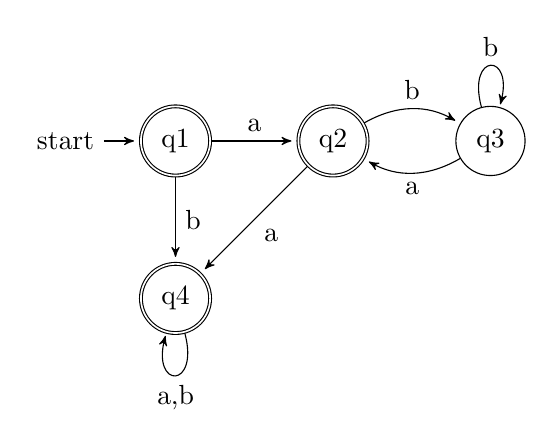
\begin{tikzpicture}[>=stealth',shorten >=2pt, auto, node distance=2cm]
    % Nodes {q1, q2, q3, q4, q5, etc}
    \node [state, initial, accepting] 		(q1) 				 {q1};
    \node [state, accepting] 	            (q2)  [right of=q1]  {q2};
    \node [state]                           (q3)  [right of=q2]  {q3};
    \node [state, accepting]				(q4)  [below of=q1]  {q4};
    
    % Paths
    \path [->] 	(q1) edge 				node	{a}		(q2);
    \path [->] 	(q1) edge 				node	{b}		(q4);
    \path [->] 	(q2) edge [bend left]	node	{b}		(q3);
    \path [->] 	(q2) edge 				node	{a}		(q4);
    \path [->] 	(q3) edge [bend left]	node	{a}		(q2);
    \path [->] 	(q3) edge [loop above] 	node	{b}		(q3);
    \path [->] 	(q4) edge [loop below] 	node	{a,b}	(q4);
    
    \end{tikzpicture} \\
\end{center}

f. \{ w $|$ w is any string not in a* $\bigcup$ b* \} \\

Simpler language
\begin{center}
    \begin{tikzpicture}[>=stealth',shorten >=2pt, auto, node distance=3cm]
    % Nodes {q1, q2, q3, q4, q5, etc}
    \node [state, initial, accepting] 		(q1) 				 {q1};
    \node [state, accepting] 	            (q2)  [right of=q1]  {q2};
    \node [state]                           (q3)  [right of=q2]  {q3};
    \node [state, accepting]				(q4)  [below of=q2]  {q4};
    
    % Paths
    \path [->] 	(q1) edge 				node	{a}		(q2);
    \path [->] 	(q1) edge 				node	{b}		(q4);
    \path [->] 	(q2) edge           	node	{b}		(q3);
    \path [->] 	(q2) edge [loop above] 	node	{a}	    (q2);
    \path [->] 	(q3) edge [loop right] 	node	{a,b}   (q3);
    \path [->] 	(q4) edge [loop below] 	node	{b}	    (q4);
    \path [->] 	(q4) edge 				node	{a}		(q3);
    
    \end{tikzpicture} \\
\end{center}

Language given
\begin{center}
    \begin{tikzpicture}[>=stealth',shorten >=2pt, auto, node distance=3cm]
    % Nodes {q1, q2, q3, q4, q5, etc}
    \node [state, initial] 		(q1) 				 {q1};
    \node [state] 	            (q2)  [right of=q1]  {q2};
    \node [state, accepting]    (q3)  [right of=q2]  {q3};
    \node [state]				(q4)  [below of=q2]  {q4};
    
    % Paths
    \path [->] 	(q1) edge 				node	{a}		(q2);
    \path [->] 	(q1) edge 				node	{b}		(q4);
    \path [->] 	(q2) edge           	node	{b}		(q3);
    \path [->] 	(q2) edge [loop above] 	node	{a}	    (q2);
    \path [->] 	(q3) edge [loop right] 	node	{a,b}   (q3);
    \path [->] 	(q4) edge [loop below] 	node	{b}	    (q4);
    \path [->] 	(q4) edge 				node	{a}		(q3);
    
    \end{tikzpicture} \\
\end{center}

g. \{ w$|$ w is any string that doesn\textsc{\char13}t contain exactly two a\textsc{\char13}s \} \\

Simpler language
\begin{center}
    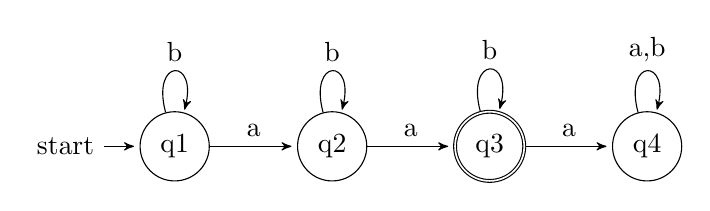
\begin{tikzpicture}[>=stealth',shorten >=2pt, auto, node distance=2cm]
    % Nodes {q1, q2, q3, q4, q5, etc}
    \node [state, initial] 		(q1) 				 {q1};
    \node [state] 				(q2)  [right of=q1]  {q2};
    \node [state, accepting]   	(q3)  [right of=q2]  {q3};
    \node [state]	            (q4)  [right of=q3]  {q4};
    
    % Paths
    \path [->] 	(q1) edge 				node	{a}		(q2);
    \path [->] 	(q1) edge [loop above] 	node	{b}		(q1);
    \path [->] 	(q2) edge 				node	{a}		(q3);
    \path [->] 	(q2) edge [loop above] 	node	{b}		(q2);
    \path [->] 	(q3) edge 				node	{a}		(q4);
    \path [->] 	(q3) edge [loop above] 	node	{b}		(q3);
    \path [->] 	(q4) edge [loop above] 	node	{a,b}	(q4);
    
    \end{tikzpicture} \\
\end{center}

Language given
\begin{center}
    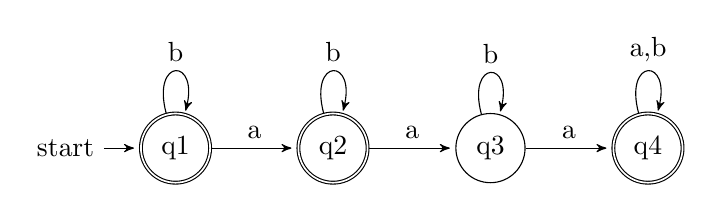
\begin{tikzpicture}[>=stealth',shorten >=2pt, auto, node distance=2cm]
    % Nodes {q1, q2, q3, q4, q5, etc}
    \node [state, initial, accepting] 		(q1) 				 {q1};
    \node [state, accepting] 				(q2)  [right of=q1]  {q2};
    \node [state]   	                    (q3)  [right of=q2]  {q3};
    \node [state, accepting]	            (q4)  [right of=q3]  {q4};
    
    % Paths
    \path [->] 	(q1) edge 				node	{a}		(q2);
    \path [->] 	(q1) edge [loop above] 	node	{b}		(q1);
    \path [->] 	(q2) edge 				node	{a}		(q3);
    \path [->] 	(q2) edge [loop above] 	node	{b}		(q2);
    \path [->] 	(q3) edge 				node	{a}		(q4);
    \path [->] 	(q3) edge [loop above] 	node	{b}		(q3);
    \path [->] 	(q4) edge [loop above] 	node	{a,b}	(q4);
    
    \end{tikzpicture} \\
\end{center}

h. \{ w$|$ w is any string except a and b \} \\

Simpler language
\begin{center}
    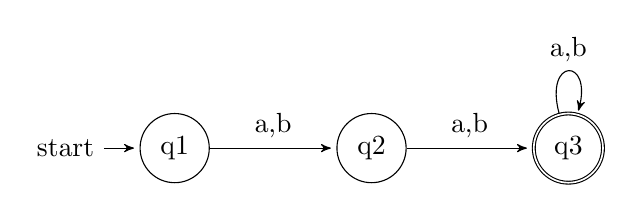
\begin{tikzpicture}[>=stealth',shorten >=2pt, auto, node distance=2.5cm]
    % Nodes {q1, q2, q3, q4, q5, etc}
    \node [state, initial] 		(q1) 				 {q1};
    \node [state] 				(q2)  [right of=q1]  {q2};
    \node [state, accepting]   	(q3)  [right of=q2]  {q3};
    
    % Paths
    \path [->] 	(q1) edge 				node	{a,b}		(q2);
    \path [->] 	(q2) edge 				node	{a,b}		(q3);
    \path [->] 	(q3) edge [loop above] 	node	{a,b}		(q3);
    
    \end{tikzpicture} \\
\end{center}

Language given
\begin{center}
    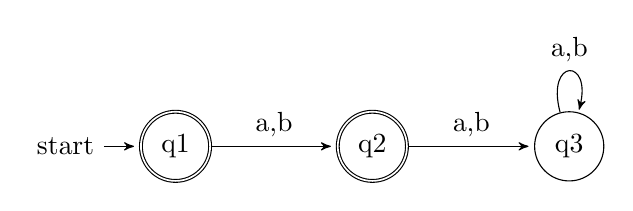
\begin{tikzpicture}[>=stealth',shorten >=2pt, auto, node distance=2.5cm]
    % Nodes {q1, q2, q3, q4, q5, etc}
    \node [state, initial, accepting] 		(q1) 				 {q1};
    \node [state, accepting] 				(q2)  [right of=q1]  {q2};
    \node [state]   	                    (q3)  [right of=q2]  {q3};
    
    % Paths
    \path [->] 	(q1) edge 				node	{a,b}		(q2);
    \path [->] 	(q2) edge 				node	{a,b}		(q3);
    \path [->] 	(q3) edge [loop above] 	node	{a,b}		(q3);
    
    \end{tikzpicture} \\
\end{center}

\noindent
1.6: a, b, c, d, e, f, g, h, I, j, k, l, m, n \\

a.
%{w| w begins with a 1 and ends with a 0}
\begin{center}
    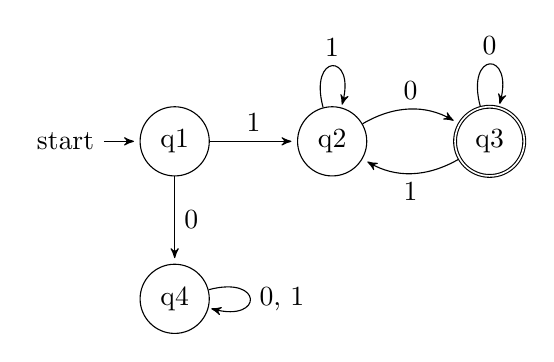
\begin{tikzpicture}[>=stealth',shorten >=2pt, auto, node distance=2cm]
    % Nodes {q1, q2, q3, q4, q5, etc}
    \node [state, initial]    	(q1) 				 {q1};
    \node [state] 				(q2)  [right of=q1]  {q2};
    \node [state, accepting]   	(q3)  [right of=q2]  {q3};
    \node [state]	            (q4)  [below of=q1]  {q4};
    
    % Paths
    \path [->] 	(q1) edge 				node	{1}		(q2);
    \path [->] 	(q1) edge 				node	{0}		(q4);
    \path [->] 	(q2) edge [bend left]	node	{0}		(q3);
    \path [->] 	(q2) edge [loop above] 	node	{1}		(q2);
    \path [->] 	(q3) edge [bend left]	node	{1}		(q2);
    \path [->] 	(q3) edge [loop above] 	node	{0}		(q3);
    \path [->] 	(q4) edge [loop right] 	node	{0, 1}	(q4);
    
    \end{tikzpicture} \\
\end{center}

b.
%{w| w contains at least three 1s}
\begin{center}
    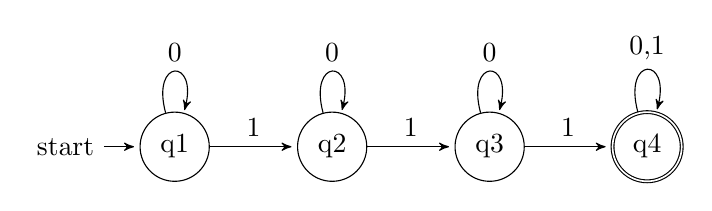
\begin{tikzpicture}[>=stealth',shorten >=2pt, auto, node distance=2cm]
    % Nodes {q1, q2, q3, q4, q5, etc}
    \node [state, initial] 		(q1) 				 {q1};
    \node [state] 				(q2)  [right of=q1]  {q2};
    \node [state]   	        (q3)  [right of=q2]  {q3};
    \node [state, accepting]	(q4)  [right of=q3]  {q4};
    
    % Paths
    \path [->] 	(q1) edge 				node	{1}		(q2);
    \path [->] 	(q1) edge [loop above] 	node	{0}		(q1);
    \path [->] 	(q2) edge 				node	{1}		(q3);
    \path [->] 	(q2) edge [loop above] 	node	{0}		(q2);
    \path [->] 	(q3) edge 				node	{1}		(q4);
    \path [->] 	(q3) edge [loop above] 	node	{0}		(q3);
    \path [->] 	(q4) edge [loop above] 	node	{0,1}	(q4);
    
    \end{tikzpicture} \\
\end{center}

c.
%{w| w contains the substring 0101 (i.e., w = x0101y for some x and y)}
\begin{center}
    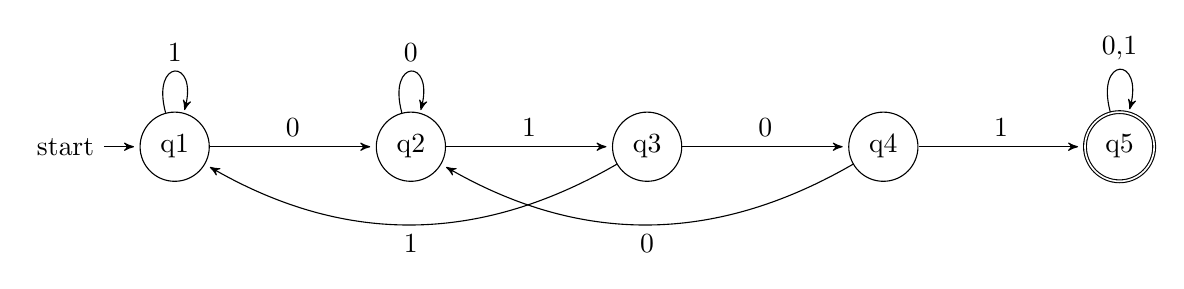
\begin{tikzpicture}[>=stealth',shorten >=2pt, auto, node distance=3cm]
    % Nodes {q1, q2, q3, q4, q5, etc}
    \node [state, initial] 		(q1) 				 {q1};
    \node [state] 				(q2)  [right of=q1]  {q2};
    \node [state]   	        (q3)  [right of=q2]  {q3};
    \node [state]   	        (q4)  [right of=q3]  {q4};
    \node [state, accepting]	(q5)  [right of=q4]  {q5};
    
    % Paths
    \path [->] 	(q1) edge 				node	{0}		(q2);
    \path [->] 	(q1) edge [loop above] 	node	{1}		(q1);
    \path [->] 	(q2) edge 				node	{1}		(q3);
    \path [->] 	(q2) edge [loop above] 	node	{0}		(q2);
    \path [->] 	(q3) edge 				node	{0}		(q4);
    \path [->] 	(q3) edge [bend left]	node	{1}		(q1);
    \path [->] 	(q4) edge 				node	{1}		(q5);
    \path [->] 	(q4) edge [bend left] 	node	{0}	    (q2);
    \path [->] 	(q5) edge [loop above] 	node	{0,1}		(q5);
    
    \end{tikzpicture} \\
\end{center}

d.
%{w| w has length at least 3 and its third symbol is a 0}
\begin{center}
    \begin{tikzpicture}[>=stealth',shorten >=2pt, auto, node distance=3cm]
    % Nodes {q1, q2, q3, q4, q5, etc}
    \node [state, initial] 		(q1) 				 {q1};
    \node [state] 				(q2)  [right of=q1]  {q2};
    \node [state]   	        (q3)  [right of=q2]  {q3};
    \node [state]   	        (q4)  [below of=q3]  {q4};
    \node [state, accepting]	(q5)  [right of=q3]  {q5};
    
    % Paths
    \path [->] 	(q1) edge 				node	{0,1}	(q2);
    \path [->] 	(q2) edge 				node	{0,1}	(q3);
    \path [->] 	(q3) edge 				node	{1}		(q4);
    \path [->] 	(q3) edge 				node	{0}		(q5);
    \path [->] 	(q4) edge [loop right] 	node	{0,1}   (q4);
    \path [->] 	(q5) edge [loop above] 	node	{0,1}   (q5);
    
    \end{tikzpicture} \\
\end{center}

e.
%{w| w starts with 0 and has odd length, or starts with 1 and has even length}
\begin{center}
    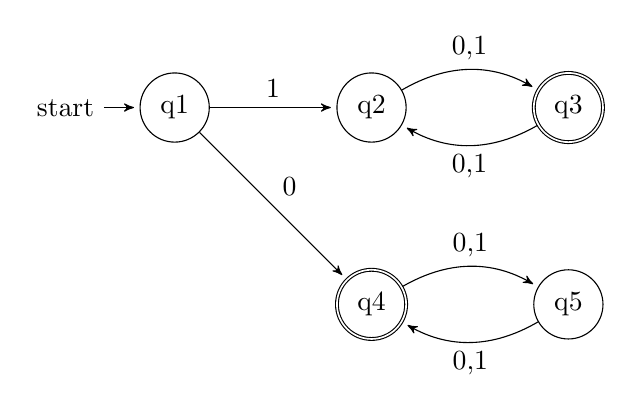
\begin{tikzpicture}[>=stealth',shorten >=2pt, auto, node distance=2.5cm]
    % Nodes {q1, q2, q3, q4, q5, etc}
    \node [state, initial] 		(q1) 				 {q1};
    \node [state] 	            (q2)  [right of=q1]  {q2};
    \node [state, accepting]    (q3)  [right of=q2]  {q3};
    \node [state, accepting]	(q4)  [below of=q2]  {q4};
    \node [state]	            (q5)  [below of=q3]  {q5};
    
    % Paths
    \path [->] 	(q1) edge 				node	{1}		(q2);
    \path [->] 	(q1) edge 				node	{0}		(q4);
    \path [->] 	(q2) edge [bend left]	node	{0,1}	(q3);
    \path [->] 	(q3) edge [bend left]	node	{0,1}	(q2);
    \path [->] 	(q4) edge [bend left]	node	{0,1}	(q5);
    \path [->] 	(q5) edge [bend left]	node	{0,1}	(q4);
    
    \end{tikzpicture} \\
\end{center}

f.
%{w| w doesn’t contain the substring 110}
\begin{center}
    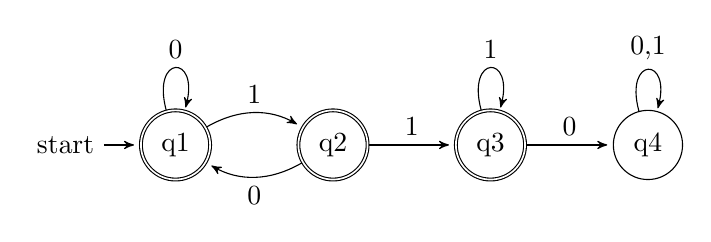
\begin{tikzpicture}[>=stealth',shorten >=2pt, auto, node distance=2cm]
    % Nodes {q1, q2, q3, q4, q5, etc}
    \node [state, initial, accepting] 		(q1) 				 {q1};
    \node [state, accepting] 				(q2)  [right of=q1]  {q2};
    \node [state, accepting]   	            (q3)  [right of=q2]  {q3};
    \node [state]	                        (q4)  [right of=q3]  {q4};
    
    % Paths
    \path [->] 	(q1) edge [bend left]	node	{1}		(q2);
    \path [->] 	(q1) edge [loop above] 	node	{0}		(q1);
    \path [->] 	(q2) edge [bend left]	node	{0}		(q1);
    \path [->] 	(q2) edge 				node	{1}		(q3);
    \path [->] 	(q3) edge 				node	{0}		(q4);
    \path [->] 	(q3) edge [loop above] 	node	{1}		(q3);
    \path [->] 	(q4) edge [loop above] 	node	{0,1}	(q4);
    
    \end{tikzpicture} \\
\end{center}

g. \\
%{w| the length of w is at most 5}
\begin{center}
    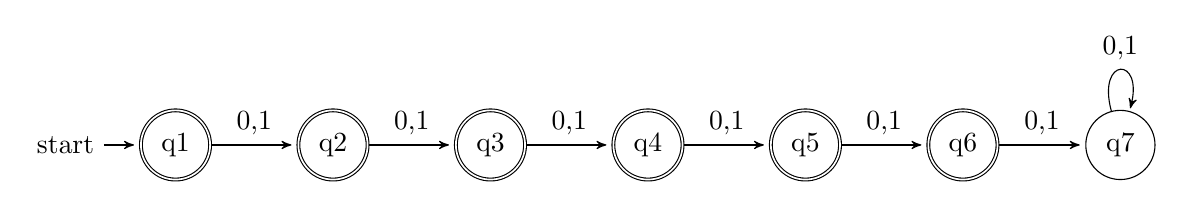
\begin{tikzpicture}[>=stealth',shorten >=2pt, auto, node distance=2cm]
    % Nodes {q1, q2, q3, q4, q5, etc}
    \node [state, initial, accepting] 		(q1) 				 {q1};
    \node [state, accepting] 				(q2)  [right of=q1]  {q2};
    \node [state, accepting]   	            (q3)  [right of=q2]  {q3};
    \node [state, accepting]   	            (q4)  [right of=q3]  {q4};
    \node [state, accepting]	            (q5)  [right of=q4]  {q5};
    \node [state, accepting]	            (q6)  [right of=q5]  {q6};
    \node [state]	                        (q7)  [right of=q6]  {q7};
    
    % Paths
    \path [->] 	(q1) edge 				node	{0,1}	(q2);
    \path [->] 	(q2) edge 				node	{0,1}	(q3);
    \path [->] 	(q3) edge 				node	{0,1}	(q4);
    \path [->] 	(q4) edge 				node	{0,1}	(q5);
    \path [->] 	(q5) edge 				node	{0,1}	(q6);
    \path [->] 	(q6) edge 				node	{0,1}	(q7);
    \path [->] 	(q7) edge [loop above] 	node	{0,1}   (q7);
    
    \end{tikzpicture} \\
\end{center}

h. \\
%{w| w is any string except 11 and 111}
\begin{center}
    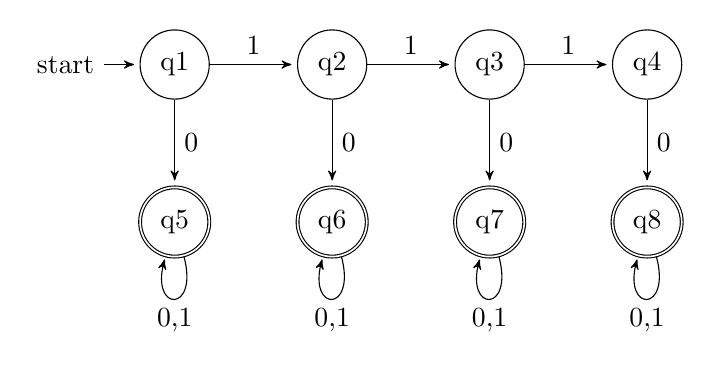
\begin{tikzpicture}[>=stealth',shorten >=2pt, auto, node distance=2cm]
    % Nodes {q1, q2, q3, q4, q5, etc}
    \node [state, initial] 		(q1) 				 {q1};
    \node [state] 				(q2)  [right of=q1]  {q2};
    \node [state]   	        (q3)  [right of=q2]  {q3};
    \node [state]	            (q4)  [right of=q3]  {q4};
    \node [state, accepting] 	(q5)  [below of=q1]  {q5};
    \node [state, accepting]    (q6)  [below of=q2]  {q6};
    \node [state, accepting] 	(q7)  [below of=q3]  {q7};
    \node [state, accepting] 	(q8)  [below of=q4]  {q8};
    
    % Paths
    \path [->] 	(q1) edge	            node	{1}		(q2);
    \path [->] 	(q2) edge 				node	{1}		(q3);
    \path [->] 	(q3) edge 				node	{1}		(q4);
    \path [->] 	(q1) edge	            node	{0}		(q5);
    \path [->] 	(q2) edge	            node	{0}		(q6);
    \path [->] 	(q3) edge	            node	{0}		(q7);
    \path [->] 	(q4) edge	            node	{0}		(q8);
    \path [->] 	(q5) edge [loop below] 	node	{0,1}	(q5);
    \path [->] 	(q6) edge [loop below] 	node	{0,1}	(q6);
    \path [->] 	(q7) edge [loop below] 	node	{0,1}	(q7);
    \path [->] 	(q8) edge [loop below] 	node	{0,1}	(q8);
    
    \end{tikzpicture} \\
\end{center}

I. \\
%{w| every odd position of w is a 1}
\begin{center}
    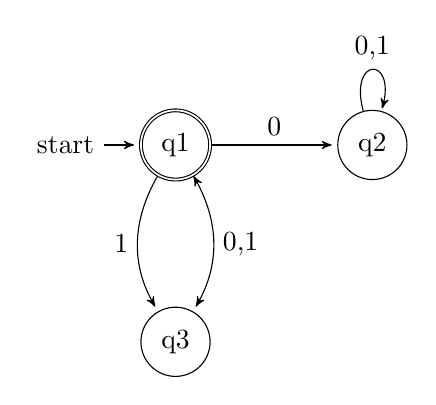
\begin{tikzpicture}[>=stealth',shorten >=2pt, auto, node distance=2.5cm]
    % Nodes {q1, q2, q3, q4, q5, etc}
    \node [state, initial, accepting] 		(q1) 				 {q1};
    \node [state] 		                    (q2) [right of=q1]	 {q2};
    \node [state] 		                    (q3) [below of=q1]	 {q3};
    
    % Paths
    \path [->] 	(q1) edge 	            node	     {0}		(q2);
    \path [->] 	(q1) edge [bend right]  node [left]	 {1}		(q3);
    \path [<->] (q1) edge [bend left]	node	     {0,1}	    (q3);
    \path [->] 	(q2) edge [loop above]	node	     {0,1}	    (q2);
    
    \end{tikzpicture} \\
\end{center}

j. \\
%{w| w contains at least two 0s and at most one 1}
\begin{center}
    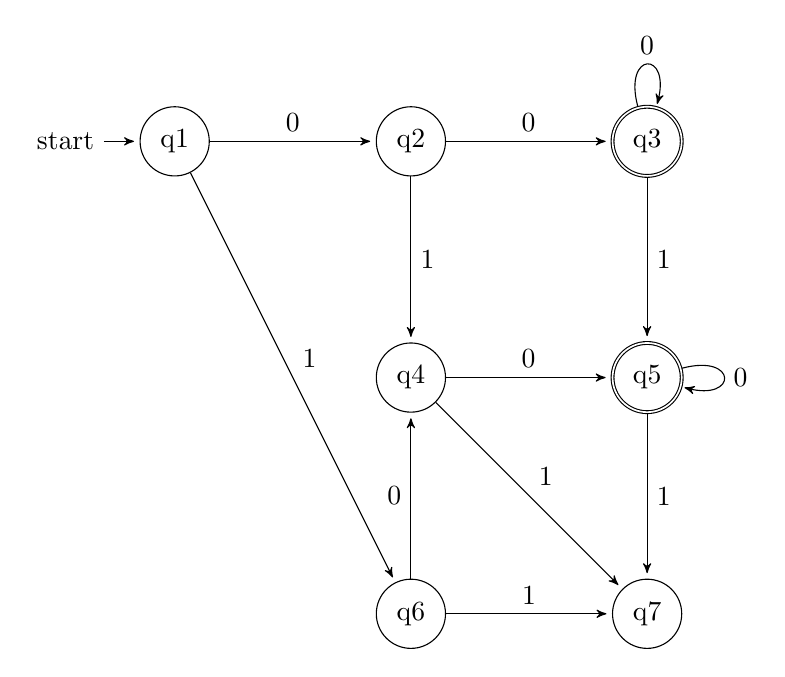
\begin{tikzpicture}[>=stealth',shorten >=2pt, auto, node distance=3cm]
    % Nodes {q1, q2, q3, q4, q5, etc}
    \node [state, initial] 		(q1) 				 {q1};
    \node [state] 				(q2)  [right of=q1]  {q2};
    \node [state, accepting]   	(q3)  [right of=q2]  {q3};
    \node [state] 	            (q4)  [below of=q2]  {q4};
    \node [state, accepting]    (q5)  [below of=q3]  {q5};
    \node [state] 	            (q6)  [below of=q4]  {q6};
    \node [state]               (q7)  [below of=q5]  {q7};
    
    % Paths
    \path [->] 	(q1) edge	            node	{0}		(q2);
    \path [->] 	(q1) edge	            node	{1}		(q6);
    \path [->] 	(q2) edge 				node	{0}		(q3);
    \path [->] 	(q2) edge 				node	{1}		(q4);
    \path [->] 	(q3) edge 				node	{1}		(q5);
    \path [->] 	(q3) edge [loop above]	node	{0}		(q3);
    \path [->] 	(q4) edge	            node	{0}		(q5);
    \path [->] 	(q4) edge	            node	{1}		(q7);
    \path [->] 	(q5) edge	            node	{1}		(q7);
    \path [->] 	(q5) edge [loop right]	node	{0}		(q5);
    \path [->] 	(q6) edge	            node	{0}		(q4);
    \path [->] 	(q6) edge	            node	{1}		(q7);
    
    \end{tikzpicture} \\
\end{center}

k. 
%{e, 0}
\begin{center}
    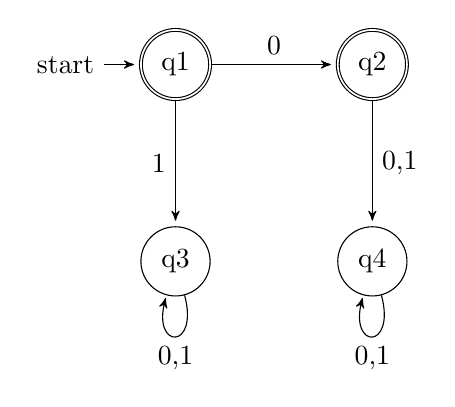
\begin{tikzpicture}[>=stealth',shorten >=2pt, auto, node distance=2.5cm]
    % Nodes {q1, q2, q3, q4, q5, etc}
    \node [state, initial, accepting] 		(q1) 				 {q1};
    \node [state, accepting]                (q2) [right of=q1]	 {q2};
    \node [state] 		                    (q3) [below of=q1]	 {q3};
    \node [state] 		                    (q4) [below of=q2]	 {q4};
    
    % Paths
    \path [->] 	(q1) edge 	            node	     {0}		(q2);
    \path [->] 	(q1) edge               node [left]	 {1}		(q3);
    \path [->] 	(q2) edge 	            node	     {0,1}		(q4);
    \path [<->] (q3) edge [loop below]	node	     {0,1}	(q3);
    \path [->] 	(q4) edge [loop below]	node	     {0,1}	(q4);
    
    \end{tikzpicture} \\
\end{center}

L. \\
%{w| w contains an even number of 0s, or contains exactly two 1s}
\begin{center}
    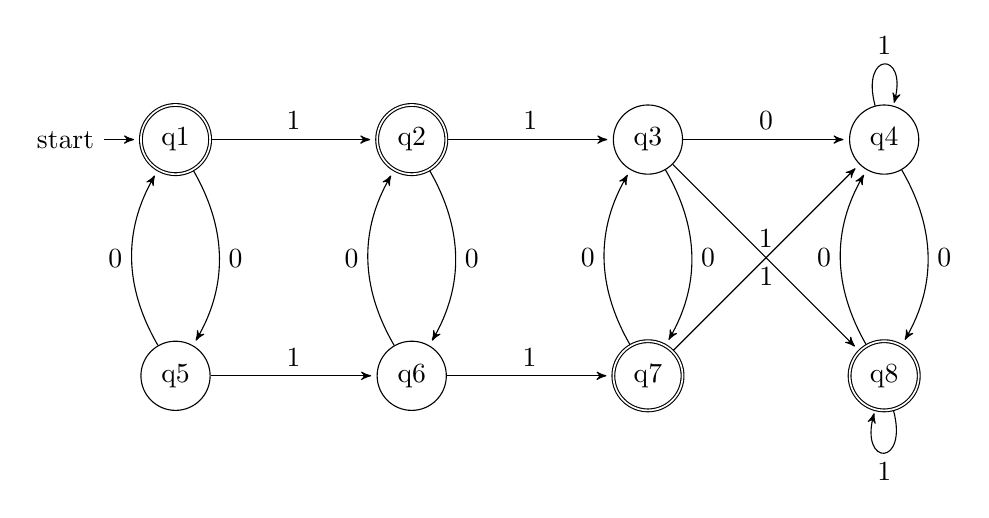
\begin{tikzpicture}[>=stealth',shorten >=2pt, auto, node distance=3
    cm]
    % Nodes {q1, q2, q3, q4, q5, etc}
    \node [state, initial, accepting] 	  (q1) 				 {q1};
    \node [state, accepting] 		      (q2)  [right of=q1]  {q2};
    \node [state]   	                  (q3)  [right of=q2]  {q3};
    \node [state]	                      (q4)  [right of=q3]  {q4};
    \node [state] 	                      (q5)  [below of=q1]  {q5};
    \node [state]                         (q6)  [below of=q2]  {q6};
    \node [state, accepting] 	          (q7)  [below of=q3]  {q7};
    \node [state, accepting] 	          (q8)  [below of=q4]  {q8};
    
    % Paths
    \path [->] 	(q1) edge	            node	        {1}		(q2);
    \path [->] 	(q2) edge 				node	        {1}		(q3);
    \path [->] 	(q3) edge 				node	        {0}		(q4);
    \path [->] 	(q3) edge 				node [above]    {1}		(q8);
    
    \path [->] 	(q5) edge	            node	        {1}		(q6);
    \path [->] 	(q6) edge 				node	        {1}		(q7);
    \path [->] 	(q7) edge 				node [below]	{1}		(q4);
    
    \path [->] 	(q1) edge [bend left]   node	        {0}		(q5);
    \path [->] 	(q2) edge [bend left]   node	        {0}		(q6);
    \path [->] 	(q3) edge [bend left]   node	        {0}		(q7);
    \path [->] 	(q4) edge [bend left]   node	        {0}		(q8);
    
    \path [->] 	(q5) edge [bend left]   node	        {0}		(q1);
    \path [->] 	(q6) edge [bend left]   node	        {0}		(q2);
    \path [->] 	(q7) edge [bend left]   node	        {0}		(q3);
    \path [->] 	(q8) edge [bend left]   node	        {0}		(q4);
    
    \path [->] 	(q4) edge [loop above] 	node	        {1}	    (q4);
    \path [->] 	(q8) edge [loop below] 	node	        {1}	    (q8);
    
    \end{tikzpicture} \\
\end{center}

m. 
%The empty set
\begin{center}
    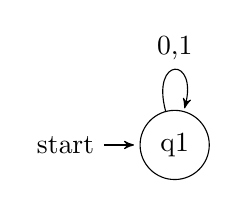
\begin{tikzpicture}[>=stealth',shorten >=2pt, auto, node distance=2cm]
    % Nodes {q1, q2, q3, q4, q5, etc}
    \node [state, initial] 		(q1) 				 {q1};
    
    % Paths
    \path [->] 	(q1) edge [loop above]	node	{0,1}		(q1);
    
    \end{tikzpicture} \\
\end{center}

n. 
%All strings except the empty string
\begin{center}
    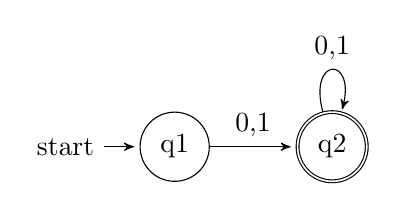
\begin{tikzpicture}[>=stealth',shorten >=2pt, auto, node distance=2cm]
    % Nodes {q1, q2, q3, q4, q5, etc}
    \node [state, initial] 		    (q1) 				 {q1};
    \node [state, accepting] 		(q2) [right of=q1]	 {q2};
    
    % Paths
    \path [->] 	(q1) edge 	            node	{0,1}		(q2);
    \path [->] 	(q2) edge [loop above]	node	{0,1}		(q2);
    
    \end{tikzpicture} \\
\end{center}

\noindent
1.7: b, c, d, e, g, h \\

b.

The language of Exercise 1.6l with six states

\{w$|$ w contains the substring 0101 (i.e., w = x0101y for some x and y)\}
\begin{center}
    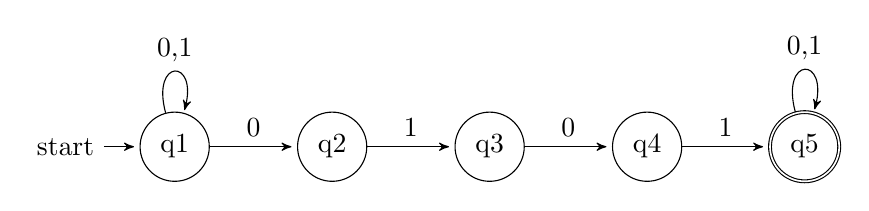
\begin{tikzpicture}[>=stealth',shorten >=2pt, auto, node distance=2cm]
    % Nodes {q1, q2, q3, q4, q5, etc}
    \node [state, initial] 		(q1) 				 {q1};
    \node [state] 				(q2)  [right of=q1]  {q2};
    \node [state]   			(q3)  [right of=q2]  {q3};
    \node [state]   			(q4)  [right of=q3]  {q4};
    \node [state, accepting]	(q5)  [right of=q4]  {q5};
    
    % Paths
    \path [->] 	(q1) edge 				node	{0}		(q2);
    \path [->] 	(q1) edge [loop above] 	node	{0,1}		(q1);
    \path [->] 	(q2) edge 				node	{1}		(q3);
    \path [->] 	(q3) edge 				node	{0}		(q4);
    \path [->] 	(q4) edge 				node	{1}		(q5);
    \path [->] 	(q5) edge [loop above] 	node	{0,1}	(q5);
    
    \end{tikzpicture} \\
\end{center}

c.

The language of Exercise 1.6l with six states
%{w| w contains an even number of 0s, or contains exactly two 1s}
\begin{center}
    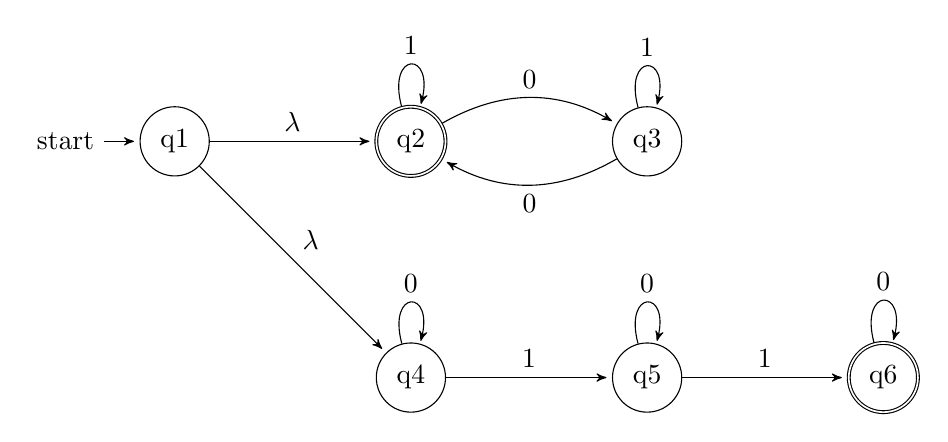
\begin{tikzpicture}[>=stealth',shorten >=2pt, auto, node distance=3cm]
    % Nodes {q1, q2, q3, q4, q5, etc}
    \node [state, initial] 		(q1) 				 {q1};
    \node [state, accepting] 	(q2)  [right of=q1]  {q2};
    \node [state]   			(q3)  [right of=q2]  {q3};
    \node [state]   			(q4)  [below of=q2]  {q4};
    \node [state]   			(q5)  [right of=q4]  {q5};
    \node [state, accepting]	(q6)  [right of=q5]  {q6};
    
    % Paths
    \path [->] 	(q1) edge 				node	{$\lambda$}		(q2);
    \path [->] 	(q1) edge 				node	{$\lambda$}		(q4);
    \path [->] 	(q2) edge [loop above] 	node	{1}     (q2);
    \path [->] 	(q2) edge [bend left]	node	{0}		(q3);
    \path [->] 	(q3) edge [bend left]	node	{0}		(q2);
    \path [->] 	(q3) edge [loop above] 	node	{1}     (q3);
    \path [->] 	(q4) edge 				node	{1}		(q5);
    \path [->] 	(q4) edge [loop above] 	node	{0}     (q4);
    \path [->] 	(q5) edge 				node	{1}		(q6);
    \path [->] 	(q5) edge [loop above] 	node	{0}	    (q5);
    \path [->] 	(q6) edge [loop above] 	node	{0}	    (q6);
    
    \end{tikzpicture} \\
\end{center}


d. The language {0} with two states
\begin{center}
    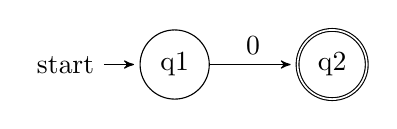
\begin{tikzpicture}[>=stealth',shorten >=2pt, auto, node distance=2cm]
    % Nodes {q1, q2, q3, q4, q5, etc}
    \node [state, initial] 		(q1) 				 {q1};
    \node [state, accepting]	(q2)  [right of=q1]  {q2};
    
    % Paths
    \path [->] 	(q1) edge 				node	{0}		(q2);
    
    \end{tikzpicture} \\
\end{center}


e. The language 0*1*0\textsuperscript{+} with three states \\
\begin{center}
    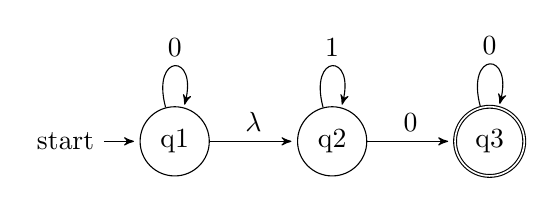
\begin{tikzpicture}[>=stealth',shorten >=2pt, auto, node distance=2cm]
    % Nodes {q1, q2, q3, q4, q5, etc}
    \node [state, initial] 		(q1) 				 {q1};
    \node [state] 		        (q2)  [right of=q1]	 {q2};
    \node [state, accepting]	(q3)  [right of=q2]  {q3};
    
    % Paths
    \path [->] 	(q1) edge 				node	{$\lambda$}	   (q2);
    \path [->] 	(q1) edge [loop above] 	node	{0}	           (q1);
    \path [->] 	(q2) edge 				node	{0}	           (q3);
    \path [->] 	(q2) edge [loop above] 	node	{1}	           (q2);
    \path [->] 	(q3) edge [loop above] 	node	{0}	           (q3);
    
    \end{tikzpicture} \\
\end{center}

g. The language \{$\epsilon$\} with one state \\
\begin{center}
    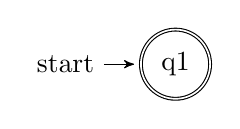
\begin{tikzpicture}[>=stealth',shorten >=2pt, auto, node distance=2cm]
    % Nodes {q1, q2, q3, q4, q5, etc}
    \node [state, initial, accepting] 		(q1) 				 {q1};
    
    % no Paths for this one.
    \end{tikzpicture} \\
\end{center}


h. The language 0* with one state \\
\begin{center}
    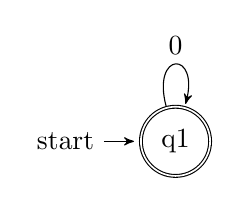
\begin{tikzpicture}[>=stealth',shorten >=2pt, auto, node distance=2cm]
    % Nodes {q1, q2, q3, q4, q5, etc}
    \node [state, initial, accepting] 		(q1) 				 {q1};
    
    % Paths
    \path [->] 	(q1) edge [loop above]	node	{0}		(q1);
    
    \end{tikzpicture} \\
\end{center}


\noindent
1.8: a, b \\
Use the construction in the proof of Theorem 1.45 to give the state \\
diagrams of NFAs recognizing the union of the languages described in \\

a. Exercises 1.6a and 1.6b \\

b. Exercises 1.6c and 1.6f \\

\noindent
1.9: a, b \\
Use the construction in the proof of Theorem 1.47 to give the state \\
diagrams of NFAs recognizing the concatenation of the languages described in \\

a. Exercises 1.6g and 1.6i \\

b. Exercises 1.6b and 1.6m \\

\noindent
1.10: a, b, c \\
Use the construction in the proof of Theorem 1.49 to give the state \\
diagrams of NFAs recognizing the star of the languages described in \\

a. Exercise 1.6b \\

b. Exercise 1.6j \\

c. Exercise 1.6m \\

\noindent
1.12 \\


\noindent
1.13 \\


\noindent
1.16 \\


\noindent
1.17: a, b \\

a. \\

b. \\

\noindent
1.18 \\

a. $1\sum\textsuperscript{*}0$ \\
%{w| w begins with a 1 and ends with a 0}

b. $\sum\textsuperscript{*}1\sum\textsuperscript{*}1\sum\textsuperscript{*}1\sum\textsuperscript{*}$ \\
%{w| w contains at least three 1s}

c. $\sum\textsuperscript{*}0101\sum\textsuperscript{*}$ \\
%{w| w contains the substring 0101 (i.e., w = x0101y for some x and y)}

d. $\sum\sum0\sum\textsuperscript{*}$ \\
%{w| w has length at least 3 and its third symbol is a 0}

e. $(0\bigcup1\sum)(\sum\sum)\textsuperscript{*}$ \\
%{w| w starts with 0 and has odd length, or starts with 1 and has even length}

f. $0\textsuperscript{*}(10\textsuperscript{+})\textsuperscript{*}1\textsuperscript{*}$ \\
%{w| w doesn’t contain the substring 110}

g. $(\epsilon\bigcup\sum)\textsuperscript{5}$ \\
%{w| the length of w is at most 5}

h. $\epsilon \bigcup \sum \bigcup 0 \sum \bigcup 10 \bigcup 0 \sum\sum \bigcup 10\sum \bigcup 110 \bigcup \sum \textsuperscript{3} \sum \textsuperscript{+} $ \\
%{w| w is any string except 11 and 111}

I. $(1 \sum) \textsuperscript{*}(\epsilon \bigcup 1) $ \\
%{w| every odd position of w is a 1}

j. $00 \textsuperscript{+} \bigcup 100 \textsuperscript{+} \bigcup 0 \textsuperscript{+}
    10 \textsuperscript{+} \bigcup 00 \textsuperscript{+} 1 $ \\
%{w| w contains at least two 0s and at most one 1}

k. $ 0 \bigcup \epsilon $ \\
%{", 0}

L. $ 1 \textsuperscript{*} (01\textsuperscript{*}01\textsuperscript{*}) \bigcup 0 
     \textsuperscript{*} 10 \textsuperscript{*} 10 \textsuperscript{*} $ \\
%{w| w contains an even number of 0s, or contains exactly two 1s}

m. $ \emptyset $ \\
%The empty set

n. $ \sum \textsuperscript{+} $ \\
%All strings except the empty string

\noindent
1.20: a, b, c, d, e, f, g, h \\

\noindent
a. \\
Members: ab, abb \\
Not members: ba, bba \\

\noindent
b. \\
Members: ab, ababab \\
Not members: aba, bab \\

\noindent
c. \\
Members: aaa, bbb \\
Not members: aabb, bbaa \\

\noindent
d. \\
Members: aaa, aaaaaa  \\
Not members: a, aaaa
 \\

\noindent
e. \\
Members: aba, bbaaabaabb \\
Not members: a, b
 \\

\noindent
f. \\
Members: aba, bab \\
Not members: ababab, ba \\

\noindent
g. \\
Members: b, ab \\
Not members: a, ba \\

\noindent
h. \\
Members: a, bbab \\
Not members: b, $\epsilon$
\\

\noindent
1.21 \\

\noindent
1.22 \\

\end{document}
